\section{Data}
\label{sec:data}

\subsection{Sources and provenance}

Table~\ref{tab:data} lists the series. The national accounts are quarterly volumes of the 2015 base, not seasonally adjusted. From 2005 they are the original DANE series; for 1993--2004 they are retropolated: GDP, consumption and investment by proportional disaggregation with seasonal profiles of the official series, and government consumption by the Denton--Cholette method \citep{Denton1971}. Employment and the informality rate come from the GEIH universe of ICML release 2.6.1 \citep{VeraJaramillo2025ICML, VeraJaramillo2026Zenodo}, aggregated from monthly to quarterly values. The informality rate is informal employment over total employment, consistent with the employment series by construction.

\begin{table}[H]
\centering
\caption{Observables and provenance.}
\label{tab:data}
\footnotesize
\begin{tabularx}{\textwidth}{L{3.6cm} L{3.7cm} Y}
\toprule
\textbf{Series} & \textbf{Source} & \textbf{Provenance by period} \\
\midrule
GDP, private consumption, gross fixed capital formation, government consumption & DANE quarterly national accounts, base 2015, chained volumes & 2005--2026: original series. 1993--2004: retropolated quarterly series. \\
Total employment & ICML 2.6.1, GEIH universe & 2001--2026: national survey (ECH and GEIH). 1993--2000: ICML reconstruction from annual survey levels of a different design. \\
Labor-informality rate & ICML 2.6.1, GEIH universe & 2021--2026: current definition. 2007--2020: inversion of published moving windows, with a bridge between definitions. 2001--2006: six aggregate anchors. 1993--2000: ICML backcast. \\
Relative labor earnings (informal / formal) & GEIH microdata, author's processing & 2007Q1--2026Q2, quarterly, by position and unit size; missing 2008Q2--Q4, 2011 and 2020Q2. Historical informality classification until 2021, current definition from 2022. \\
\bottomrule
\end{tabularx}
\end{table}

The provenance matters for the interpretation of the results. The quarterly dynamics of employment and informality before 2001 are generated by the ICML reconstruction, and the informality rate before 2007 is anchored to few observations. The estimation uses all quarters, which is the purpose of the reconstruction; Section~\ref{sec:identification} reports how much of the information about the size of the informal sector comes from each period.

\subsection{Relative labor earnings}

The earnings series is built from the monthly GEIH microdata processed by the author (January 2007 to August 2026). Each employed person is classified as formal or informal with the same rules that underlie the informality series: a size-and-position proxy until 2021 and the social-security-based definition from 2022, with persons whose status cannot be determined left unclassified rather than imputed. For workers with positive labor income, excluding unpaid family workers, the monthly weighted sums of income and of persons are computed with the national expansion factor of the survey, and the quarterly ratio is the weighted mean income of informal workers divided by that of formal workers. Income is DANE's derived labor income (main and secondary jobs) from mid-2008 and the sum of the main-job wage or profit and secondary-job income before. An alternative ratio uses income per hour worked.

Because the labor-only accounting of Section~\ref{sec:model} treats informal income as value added, the series is also computed by group of worker. On average over 2007--2026, 68.6\% of paid informal workers are own-account workers or employers, 22.3\% are employees in units of up to five persons, 5.6\% are domestic employees and 3.4\% are employees of units with six or more persons; the size question (P6870 until 2021, P3069 afterwards) is answered by all employees. The interpretation of these earnings differs by employment position. Income of own-account workers and employers includes a mixed-income component, whereas an employee's wage captures labor compensation but not the enterprise's entire value added. The baseline uses a group-specific \emph{proxy} for informal value added per worker: reported income for the first three groups and the wage divided by $1-\alpha$ for employees of larger units, who are assumed to work with the firm's capital. In particular, treating earnings of domestic workers and employees of small units as their entire attributable value added is an identifying approximation, not an accounting identity observed in the survey. The resulting proxy is divided by the mean wage of formal employees; formal own-account workers are excluded from the denominator because their income is not a wage. This adjustment changes the sample-average ratio from 0.421 (unadjusted) to 0.441. Section~\ref{sec:limitations} discusses its limitations.

The survey asks wage earners for their pay ``before deductions'', so the employee's own contributions are included in the reported wage. The difference between the reported wage and the employer's total labor cost, which is what the model's gross formal wage $(1-\alpha)Y_f/N_f$ measures, consists of the employer's social-security contributions, the payroll contributions (\emph{parafiscales}) and the social benefits paid outside the monthly wage. These are set by law and are computed quarter by quarter for a worker earning less than ten minimum wages: pension (employer share 11.6\% in 2007 and 12\% from 2008), health (8.5\%), occupational risk (0.5\%), family compensation fund (4\%), the payroll contributions to SENA and ICBF (5\%), and the benefits (service bonus, severance pay and its interest, and holidays, 21.8\%). The 2012 tax reform (Law 1607) removed the SENA and ICBF contributions from May 2013 and the employer's health contribution from January 2014 for these workers. Non-wage costs therefore fall from 51.9\% of the wage in 2008--2012 to 38.4\% from 2014. Let $d_t^{\mathrm{nw}}$ be the employer non-wage cost premium relative to the reported wage. Its log gross-up, $\ln(1+d_t^{\mathrm{nw}})$, converts the reported formal wage into labor cost in the measurement equation of Section~\ref{sec:identification}; a sensitivity uses contributions only, for the case in which reported income already includes the benefits.

The ratio is stable between 0.42 and 0.47 from 2007 to 2019, falls during the pandemic and drops to about 0.37 when the current definition of informality is introduced in 2022 (Figure~\ref{fig:earnings}). The drop coincides with the change of definition, when the share of unclassified workers falls from about 3.5\% to almost zero, and is treated as a level shift in the measurement equation. Twenty-one months of 2008 and 2011 lack a usable expansion factor in the normalized files and are missing, as are March and April 2020, when telephone collection left a quarter of the employed without a formality status; quarters require three valid months.

\begin{figure}[H]
\centering
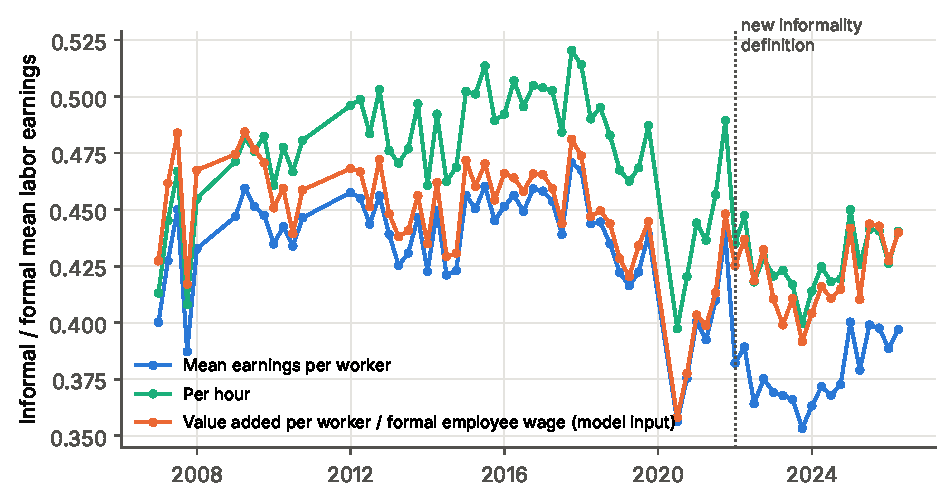
\includegraphics[width=0.85\textwidth]{fig_earnings.pdf}
\caption{Ratio of mean labor earnings of informal to formal workers, GEIH, 2007Q1--2026Q2. The dotted line marks the change in the definition of informality.}
\label{fig:earnings}
\end{figure}

\subsection{Transformations}

Let $Y_t$, $C_t$, $I_t$, $G_t$ and $N_t$ denote the levels and $s_t$ the informality rate. The observables are
\begin{equation}
\bm{y}^{\mathrm{obs}}_t = \big(\Delta\ln Y_t,\ \Delta\ln C_t,\ \Delta\ln I_t,\ \Delta\ln G_t,\ \Delta\ln N_t,\ \Delta\logit s_t\big)^{\top} - \bm{m}_{q(t)},
\label{eq:obs}
\end{equation}
where $\bm{m}_{q}$ is the mean of each growth rate in quarter of the year $q\in\{1,2,3,4\}$ over 2005--2018. Removing quarter-specific means removes deterministic seasonality and the mean growth rate together; the same means are applied to the whole sample. The earnings ratio enters in logarithmic \emph{levels}, $\ln R_t$, because its level is what identifies relative productivity. In the labor-only estimates the logit informality rate also enters in levels, as a deviation from the logit of its sample mean with the quarter-of-year pattern of 2005--2018 removed (Section~\ref{sec:identification}). The sample runs from 1993Q2 to 2026Q2 (133 quarters). The quarters 2020Q2--2020Q4, spanning the unprecedented contraction in output and employment and a change in survey collection mode, are treated as missing in the likelihood. The choice avoids asking a first-order Gaussian approximation to accommodate those exceptional observations, but it also means that the paper does not estimate the pandemic adjustment mechanism.

Two features of the data shape the estimation. First, quarterly growth rates have almost no persistence: excluding the pandemic quarters, the first-order autocorrelation is $-0.13$ for GDP, $0.06$ for consumption and $-0.21$ for employment, so no model can predict them much better than their mean. Second, the growth of investment and of the logit informality rate is negatively autocorrelated ($-0.45$ and $-0.37$), the signature of noise in levels.
